\documentclass[12pt]{article}

\usepackage{sbc-template}
\usepackage{graphicx,url}
\usepackage[utf8]{inputenc}
\usepackage[brazil]{babel}
%\usepackage[latin1]{inputenc}  

     
\sloppy

\title{Classificação de Acidentes Rodoviários a Partir de Fatores de Tráfego e Pavimento}

\author{Augusto D. N. Oliveira\inst{1}, Vitor Uchikawa\inst{2}}

\address{
    Universidade Federal de Santa Catarina (UFSC) -- Campus Joinville\\
    Programa de Pós-Graduação em Engenharia de Sistemas Eletrônicos (PPGESE)\\
    Joinville -- SC -- Brazil
    \email{augusto-\_-14@hotmail.com, vitor.uchikawa@gmail.com}
}

\begin{document} 

\maketitle

\begin{abstract}
\end{abstract}
     
\begin{resumo} 
\end{resumo}

\section{Introdução}

\subsection{Contextualização}

A classificação dos acidentes rodoviários envolve características do condutor, da via, do ambiente e da própria ocorrência \cite{who2023roadsafety}. Para examinar as relações entre essas características e o desfecho registrado, é necessário reunir informações de diferentes dimensões do sistema rodoviário.

Nesse sentido, os dados abertos da Polícia Rodoviária Federal (PRF) apresentam informações sobre localização, causa, tipo de acidente, fase do dia, condições meteorológicas e características da pista \cite{prf_dados_abertos}. Esses registros, organizados em nível de ocorrência, constituíram a principal fonte de dados utilizada neste trabalho.

Embora reúna informações detalhadas sobre os acidentes, a base da PRF não contempla todos os fatores pertinentes à predição da classificação, como aspectos relacionados ao tráfego e à conservação das rodovias. Por esse motivo, ela foi complementada com o volume de veículos nas praças de pedágio, fornecido pela Agência Nacional de Transportes Terrestres (ANTT) \cite{antt_dados_abertos}, e com o Índice de Condição da Manutenção (ICM), disponibilizado pelo Departamento Nacional de Infraestrutura de Transportes (DNIT) \cite{dnit_icm}.

A partir dessa integração, foram considerados os registros de acidentes disponíveis posteriores a 1º de novembro de 2023. Cada ocorrência foi associada, quando disponíveis, ao volume mensal da praça de pedágio mais próxima e ao ICM do trecho correspondente.

Após o pré-processamento, o conjunto de dados foi consolidado em 187.348 registros de acidentes com 13 variáveis preditoras. Nesse conjunto, a classificação do acidente foi definida como variável-alvo e dividida em três classes: com vítimas fatais, com vítimas feridas e sem vítimas.

Para representar as diferentes dimensões presentes na base, foram selecionadas variáveis relacionadas ao tipo e à causa do acidente, à fase do dia, à condição meteorológica, ao tipo de pista, ao traçado da via, ao trecho da rodovia, ao volume de pedágio e ao ICM. A partir dessas informações, também foram construídas variáveis para representar a presença de fator humano, a inclinação da via e sua geometria horizontal.

Com o conjunto de dados estruturado, a análise estatística foi utilizada para examinar as associações entre as variáveis selecionadas e a classificação dos acidentes. Em seguida, o algoritmo CatBoost foi empregado para realizar a classificação multiclasse e estimar a importância das variáveis, com tratamento direto dos atributos categóricos \cite{prokhorenkova2018catboost}.

\subsection{Problema de pesquisa}

A composição do conjunto de dados apresenta desafios que devem ser considerados durante a modelagem. Entre eles, está o desbalanceamento das classes, pois os acidentes com vítimas feridas representam a maior parte dos registros, enquanto os acidentes com vítimas fatais são menos frequentes.

Essa diferença na quantidade de registros favorece a classe majoritária durante o treinamento. Como consequência, o modelo pode apresentar desempenho global elevado e, ao mesmo tempo, ter dificuldade em reconhecer as classes com menor número de ocorrências.

Além do desbalanceamento, a definição das variáveis preditoras requer atenção ao vazamento do alvo. Informações disponibilizadas acerca de mortos e feridos revelariam ao modelo dados diretamente relacionados ao desfecho, comprometendo a avaliação.

Mesmo após a exclusão dessas variáveis, as relações observadas nos dados devem ser interpretadas como associações estatísticas, e não como relações de causa e efeito. Uma característica pode estar associada à classificação do acidente sem necessariamente explicar o desfecho observado.

Considerando essas limitações, o problema de pesquisa consiste em avaliar em que medida as características dos acidentes e das rodovias permitem distinguir as três classes analisadas. Também se busca identificar quais variáveis apresentam maior associação com a classificação e maior contribuição para o desempenho do modelo.

\subsection{Objetivo geral}

Diante disso, o objetivo geral deste trabalho é analisar as relações entre as características dos acidentes rodoviários e sua classificação. Pretende-se ainda desenvolver e avaliar um modelo de aprendizado de máquina para classificar as ocorrências registradas pela PRF e identificar as variáveis de maior relevância preditiva.

\subsection{Objetivos específicos}

\begin{itemize}
\item integrar e padronizar os dados de acidentes da PRF, de volume de pedágio da ANTT e de condição do pavimento do DNIT;

\item associar aos registros de acidentes o volume mensal da praça de pedágio mais próxima e o ICM do trecho correspondente;

\item examinar a estrutura, a qualidade, os valores ausentes e a consistência dos dados;

\item caracterizar a distribuição das classes e a distribuição espacial dos acidentes;

\item selecionar e construir as variáveis preditoras, excluindo as informações que causam vazamento do alvo;

\item medir a associação entre as variáveis categóricas e a classificação dos acidentes por meio do V de Cramér;

\item estimar a incerteza das proporções de acidentes fatais por meio do intervalo de Wilson;

\item comparar as variáveis numéricas entre as classes com o teste de Kruskal--Wallis e o tamanho de efeito epsilon ao quadrado;

\item examinar as relações entre as variáveis numéricas por meio da correlação de Spearman;

\item treinar e ajustar um classificador CatBoost, considerando o desbalanceamento entre as classes;

\item avaliar o modelo por meio da acurácia, acurácia balanceada, F1 macro, F1 ponderado, métricas por classe e matriz de confusão; e

\item identificar as variáveis mais importantes para a classificação produzida pelo modelo.

\end{itemize}

\section{General Information}

All full papers and posters (short papers) submitted to some SBC conference,
including any supporting documents, should be written in English or in
Portuguese. The format paper should be A4 with single column, 3.5 cm for upper
margin, 2.5 cm for bottom margin and 3.0 cm for lateral margins, without
headers or footers. The main font must be Times, 12 point nominal size, with 6
points of space before each paragraph. Page numbers must be suppressed.

Full papers must respect the page limits defined by the conference.
Conferences that publish just abstracts ask for \textbf{one}-page texts.

\section{First Page} \label{sec:firstpage}

The first page must display the paper title, the name and address of the
authors, the abstract in English and ``resumo'' in Portuguese (``resumos'' are
required only for papers written in Portuguese). The title must be centered
over the whole page, in 16 point boldface font and with 12 points of space
before itself. Author names must be centered in 12 point font, bold, all of
them disposed in the same line, separated by commas and with 12 points of
space after the title. Addresses must be centered in 12 point font, also with
12 points of space after the authors' names. E-mail addresses should be
written using font Courier New, 10 point nominal size, with 6 points of space
before and 6 points of space after.

The abstract and ``resumo'' (if is the case) must be in 12 point Times font,
indented 0.8cm on both sides. The word \textbf{Abstract} and \textbf{Resumo},
should be written in boldface and must precede the text.

\section{CD-ROMs and Printed Proceedings}

In some conferences, the papers are published on CD-ROM while only the
abstract is published in the printed Proceedings. In this case, authors are
invited to prepare two final versions of the paper. One, complete, to be
published on the CD and the other, containing only the first page, with
abstract and ``resumo'' (for papers in Portuguese).

\section{Sections and Paragraphs}

Section titles must be in boldface, 13pt, flush left. There should be an extra
12 pt of space before each title. Section numbering is optional. The first
paragraph of each section should not be indented, while the first lines of
subsequent paragraphs should be indented by 1.27 cm.

\subsection{Subsections}

The subsection titles must be in boldface, 12pt, flush left.

\section{Figures and Captions}\label{sec:figs}


Figure and table captions should be centered if less than one line
(Figure~\ref{fig:exampleFig1}), otherwise justified and indented by 0.8cm on
both margins, as shown in Figure~\ref{fig:exampleFig2}. The caption font must
be Helvetica, 10 point, boldface, with 6 points of space before and after each
caption.

\begin{figure}[ht]
\centering
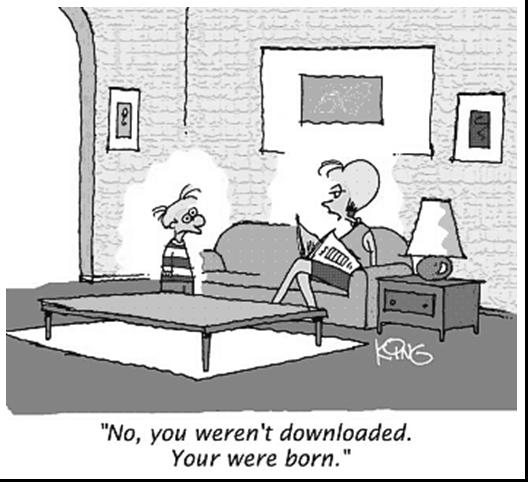
\includegraphics[width=.5\textwidth]{fig1.jpg}
\caption{A typical figure}
\label{fig:exampleFig1}
\end{figure}

\begin{figure}[ht]
\centering
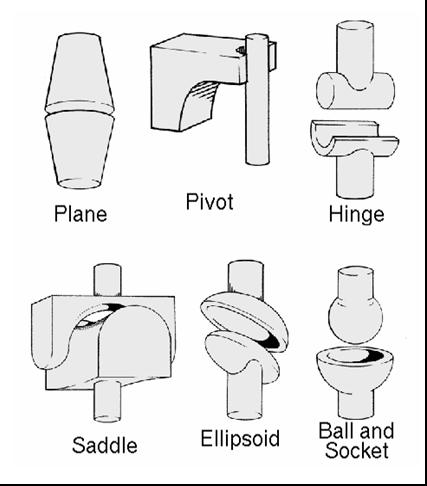
\includegraphics[width=.3\textwidth]{fig2.jpg}
\caption{This figure is an example of a figure caption taking more than one
  line and justified considering margins mentioned in Section~\ref{sec:figs}.}
\label{fig:exampleFig2}
\end{figure}

In tables, try to avoid the use of colored or shaded backgrounds, and avoid
thick, doubled, or unnecessary framing lines. When reporting empirical data,
do not use more decimal digits than warranted by their precision and
reproducibility. Table caption must be placed before the table (see Table 1)
and the font used must also be Helvetica, 10 point, boldface, with 6 points of
space before and after each caption.

\begin{table}[ht]
\centering
\caption{Variables to be considered on the evaluation of interaction
  techniques}
\label{tab:exTable1}
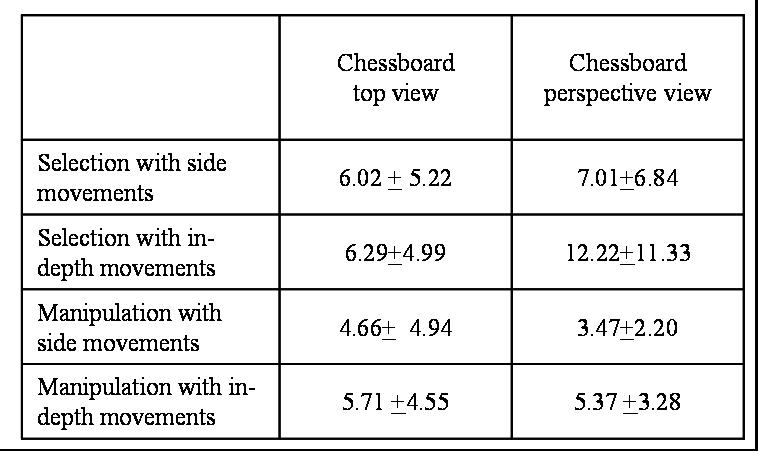
\includegraphics[width=.7\textwidth]{table.jpg}
\end{table}

\section{Images}

All images and illustrations should be in black-and-white, or gray tones,
excepting for the papers that will be electronically available (on CD-ROMs,
internet, etc.). The image resolution on paper should be about 600 dpi for
black-and-white images, and 150-300 dpi for grayscale images.  Do not include
images with excessive resolution, as they may take hours to print, without any
visible difference in the result. 

\section{References}

Bibliographic references must be unambiguous and uniform.  We recommend giving
the author names references in brackets, e.g. \cite{knuth:84},
\cite{boulic:91}, and \cite{smith:99}.

The references must be listed using 12 point font size, with 6 points of space
before each reference. The first line of each reference should not be
indented, while the subsequent should be indented by 0.5 cm.

\bibliographystyle{sbc}
\bibliography{sbc-template}

\end{document}
